
\section{Algoritmi}
\label{cap:algorithms}

\subsection{MST2Approximation}

MST2Approximation è l'implementazione dell'algoritmo di $2$-approssimazione basato sul Minimum Spanning Tree visto a lezione. L'algoritmo prevede i seguenti step:

\begin{enumerate}
    \item Selezionare un vertice radice $root$ arbitrario;
    \item Ricavare l'MST del grafo in input a partire da $root$, utilizzando ad esempio l'algoritmo di Prim;
    \item Eseguire una visita pre-order dell'MST ricavato al passo precedente;
    \item Aggiungere la radice $root$ pre-order alla fine della lista ritornata dalla visita pre-order.
    \item Calcolare il peso totale del circuito ricavato nei 2 passi precedenti e restituire il risultato.
\end{enumerate}

\noindent Il listato \ref{listing:tsp2approx} contiene la nostra implementazione dell'algoritmo, step per step.\\

\begin{listing}[!ht]
\begin{minted}{c++}
    // MST2Approximation/approx_tsp.h

    // Step 1
    random_generator::IntegerRandomGenerator random(0, distance_matrix.size() - 1);
    const size_t root = random();

    // Step 2
    std::vector<Edge> mst(mst::prim_binary_heap_mst(distance_matrix, root));

    // Step 3, 4
    DFS dfs(std::move(mst));
    const auto circuit = dfs.preorder_traversal_rec();

    // Funzione lambda che calcola la distanza tra due vertici
    const auto get_distance = [&distance_matrix](const size_t x, const size_t y) {
        return distance_matrix.at(x, y);
    };

    // Step 5
    return utils::sum_weights_in_circuit(circuit.cbegin(), circuit.cend(), get_distance);
\end{minted}
\caption{Implementazione di TSP 2-approssimato. I commenti del file originale sono stati omessi per una maggiore compattezza.}
\label{listing:tsp2approx}
\end{listing}

\noindent L'algoritmo TSP 2-approssimato è stato implementato a partire dallo pseudo codice visto in classe. \\

\subsubsection{Osservazioni}

\begin{itemize}
    \item Abbiamo usato l'algoritmo di Prim perché è più adatto rispetto a Kruskal quando il grafo è rappresentato come matrice di adiacenza. Kruskal infatti richiede di estrarre la lista di lati ordinata in modo ascendente rispetto al peso all'inizio dell'algoritmo, mentre Prim richiede di estrarre solo la lista dei vertici. Ricordiamo che in un grafo completo vale l'equivalenza \complexityCompleteGraph{}.

    \item La coda di priorità usata dall'algoritmo di Prim è stata implementata con una Min Heap binaria, la quale è già stata descritta in dettaglio nella relazione del primo progetto.
\end{itemize}

\subsection{HeldKarp}

Riportiamo lo pseudocodice dell'algortimo di programmazione dinamica Held \& Karp visto in classe. La funzione \codeinline{HeldKarp(S, v)} vista a lezione funziona nel seguente modo:

\begin{enumerate}
    \item Caso base 1: verifica se il percorso parziale $S$ contenga un solo nodo, e in caso positivo restituisce la distanza tra il nodo $v$ e il nodo di partenza $0$.
    \item Caso base 2: controlla se la distanza tra i nodi $0$ e $v$, passando per tutti i nodi in $S$, sia già stata calcolata, e in caso positivo restituisce tale valore.
    \item Caso ricorsivo:
    \begin{enumerate}
        \item Step a: Inizializza la distanza minima a $\infty$ e considera $S \setminus {v}$.
        \item Step b: Scansiona tutti i nodi in $S \setminus {v}$, calcolando ricorsivamente la distanza. Se la distanza trovata è inferiore a quelle precedentemente ricavate, viene sostituita.
        \item Step c: Verifica se il timeout è scaduto. In caso positivo, effettua l'unrolling prematuro dello stack di ricorsione e ritorna il miglior risultato ottenuto fino a questo punto.
    \end{enumerate}
    \item Step d: Ritorna la distanza minima calcolata del circuito parziale $S$.
\end{enumerate}

\noindent La nostra implementazione usa due diverse strutture dati per rappresentare il sottoinsieme $S$ tra quelle viste in \ref{held-karp-S-repr}:

\begin{itemize}
    \item \mintinline{c++}{unsigned long long} manipolati tramite bit masking se il grafo in input ha meno di 64 nodi;
    \item \mintinline{c++}{DynamicBitMask} altrimenti.
\end{itemize}

\noindent Il listato \ref{listing:held-karp} contiene la nostra implementazione dell'algoritmo, step per step.

\begin{listing}[!ht]
\begin{minted}{c++}
// HeldKarp/HeldKarp.h
using ull = unsigned long long;
using held_karp_dp_bits_t = std::unordered_map<std::pair<ull, size_t>, int>;

int held_karp_tsp_rec_bits_helper(timeout::timeout_signal& signal,
                                  DistanceMatrix<int>& distance_matrix,
                                  held_karp_dp_bits_t& C,
                                  ull bits, size_t v = 0) {
    // Caso base 1
    if (utils::is_singleton(bits, v)) {
        return distance_matrix.at(v, 0);
    }

    // Case base 2
    if (C.count({bits, v})) {
        return C[{bits, v}];
    }

    // Step a
    int min_dist = std::numeric_limits<int>::max();
    const ull difference = utils::reset_bit(bits, v);
    const size_t n = distance_matrix.size();

    // Step b
    utils::for_each(difference, n, [&](const size_t bit) {
        int dist = held_karp_tsp_rec_bits_helper(signal, distance_matrix, C,
                                                 difference, bit);
        int tmp_dist = dist + distance_matrix.at(v, bit);

        if (tmp_dist < min_dist) {
            min_dist = tmp_dist;
        }

        // Step c
        return !signal.is_expired();
    });

    // Step d
    C[{bits, v}] = min_dist;
    return min_dist;
}

\end{minted}
\caption{Implementazione di Held e Karp con BitMasking. I commenti del file originale sono stati omessi per una maggiore compattezza.}
\label{listing:held-karp}
\end{listing}

\subsubsection{Osservazioni}

\begin{itemize}
    \item Abbiamo voluto riportare qui la versione con BitMasking a 64 bit, la versione con DynamicBitMasking è simile. Il controllo su quale delle due implementazioni usare è fatto prima di lanciare la funzione di ricorsione appropriata.\\
\end{itemize}

\newpage

\subsection{Closest Insertion}
\label{sec:closest-insertion}

\emph{Closest Insertion} è una delle euristiche impiegabili per la
risoluzione problema del TSP in modo approssimato. Questa euristica
è molto simile a \emph{Farthest Insertion} (si veda \ref{sec:farthest-insertion}),
infatti differisce da essa solo per la selezione del vertice $k$
da inserire nel circuito parziale $C$.

In particolare, in questo caso viene scelto il vertice $k$ non presente
nel circuito $C$ che minimizza $\delta (k, C) = \min_{h \in C} w(h, k)$.
Sostanzialmente viene scelto il vertice $k$ più vicino al ciclo $C$,
ma che non è ancora incluso in esso.

\subsubsection{Implementazione}

Il codice è sostanzialmente simile a quello riportato nel listato
\ref{listing:farthest-insertion}, con la differenza che per
\emph{Closest Insertion} si effettua la scelta del nuovo nodo
con \mintinline{c++}{utils::select_new_k} passandogli come quarto
argomento un comparatore che permette, in questo caso, di
minimizzare $\delta (k, C)$.

\begin{listing}[!ht]
\begin{minted}{c++}
// the comparator will be passed to std::max_element.
const auto min_comparator = [](const auto& x, const auto& y) {
    return x.second > y.second;
};
\end{minted}
\caption{Differenza di implementazione per Closest Insertion rispetto a Farthest Insertion.}
\label{listing:closest-insertion-diff}
\end{listing}

\subsubsection{Approssimazione}

Questa euristica permette di trovare una soluzione $\log(n)$-approssimata,
ma è possibile dimostrare che il fattore di approssimazione può essere
ulteriormente abbassato fino ad avere una soluzione $2$-approssimata.

I risultati che abbiamo ottenuto con closest insertion sono illustrati
dalla tabella \ref{table:closest-insertion-runtime-accuracy} e dal grafico
\ref{fig:closest-insertion-accuracy-error}.

\begin{figure}[H]
    \centering

    \begin{tabular}{lrrrr}
    \toprule
    \multicolumn{5}{c}{Closest Insertion} \\
    \hline
    Instance & Exact & Solution &   Time (ms) &   Error (\%) \\
    \hline
    burma14.tsp   &     3323 &       3664 &          35 &       10.26 \\
    ulysses16.tsp &     6859 &       7054 &          36 &        2.84 \\
    ulysses22.tsp &     7013 &       7499 &          36 &        6.93 \\
    eil51.tsp     &      426 &        480 &          37 &       12.68 \\
    berlin52.tsp  &     7542 &       8626 &          35 &       14.37 \\
    kroA100.tsp   &    21282 &      24661 &          38 &       15.88 \\
    kroD100.tsp   &    21294 &      22998 &          38 &        8    \\
    ch150.tsp     &     6528 &       7763 &          40 &       18.92 \\
    gr202.tsp     &    40160 &      45660 &          46 &       13.7  \\
    gr229.tsp     &   134602 &     163597 &          52 &       21.54 \\
    pcb442.tsp    &    50778 &      58297 &         142 &       14.81 \\
    d493.tsp      &    35002 &      40537 &         180 &       15.81 \\
    dsj1000.tsp   & 18659688 &   22510610 &        1127 &       20.64 \\
    \bottomrule
    \end{tabular}

    \caption{ClosestInsertion runtime and accuracy error}
    \label{table:closest-insertion-runtime-accuracy}
\end{figure}

\begin{figure}[H]
    \centering

    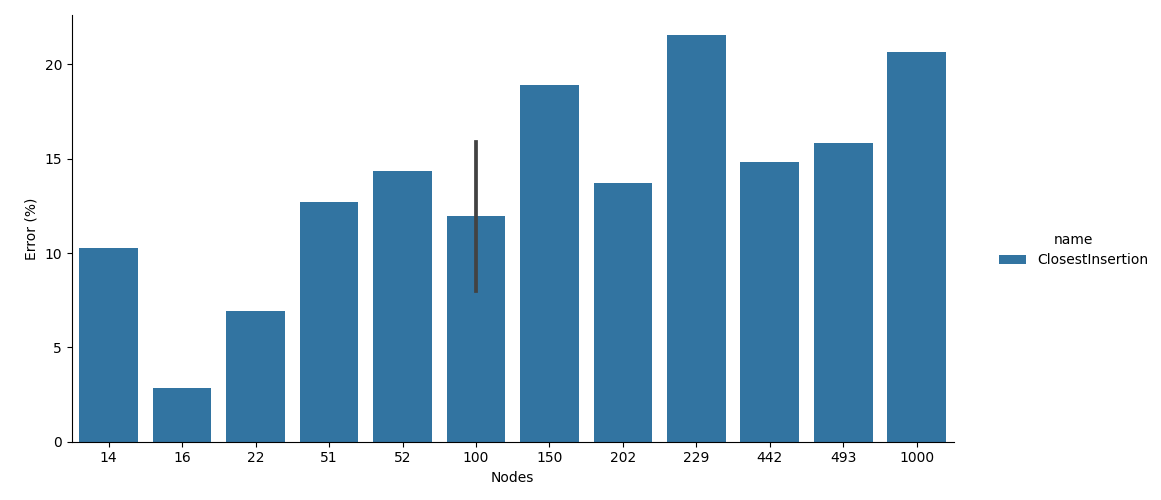
\includegraphics[width=0.9\textwidth]{./images/ClosestInsertion__approximation_error_.png}

    \caption{ClosestInsertion accuracy error scaling by nodes}
    \label{fig:closest-insertion-accuracy-error}
\end{figure}

\subsubsection{Osservazioni}

Data la netta dualità con FarthestInsertion, è doveroso analizzare
le differenze tra i due algoritmi. Dalla tabella
\ref{table:closest-farthest-insertion-runtime-accuracy}
e dal grafico \ref{fig:closest-farthest-insertion-accuracy-error}
è possibile notare che per quanto riguarda il runtime i due algoritmi
sono perfettamente alla pari, infatti minimizzare o massimizzare la
funzione $\delta (k, C)$ dal punto di vista del tempo di esecuzione
non comporta differenze. Dal punto di vista dell'errore di
approssimazione invece FarthestInsertion riesce a fare mediamente
meglio di ClosestInsertion. Da sottolineare anche il fatto che
FarthestInsertion riesce ad eliminare completamente l'errore di
approssimazione su istanze molto piccole.

\begin{figure}[H]
    \centering

    \begin{tabular}{lrrrrrr}
    \toprule
    \multicolumn{1}{c}{ } & \multicolumn{3}{c}{Closest Insertion} & \multicolumn{3}{c}{Farthest Insertion} \\
    \hline
    Instance & Solution &   Time (ms) &   Error (\%) & Solution &   Time (ms) &   Error (\%) \\
    \hline
    burma14.tsp   &     3664 &          35 &       10.26 &       3323 &          35 &        0    \\
    ulysses16.tsp &     7054 &          36 &        2.84 &       6859 &          35 &        0    \\
    ulysses22.tsp &     7499 &          36 &        6.93 &       7013 &          35 &        0    \\
    eil51.tsp     &      480 &          37 &       12.68 &        439 &          36 &        3.05 \\
    berlin52.tsp  &     8626 &          35 &       14.37 &       8118 &          36 &        7.64 \\
    kroA100.tsp   &    24661 &          38 &       15.88 &      23373 &          36 &        9.83 \\
    kroD100.tsp   &    22998 &          38 &        8    &      22577 &          36 &        6.03 \\
    ch150.tsp     &     7763 &          40 &       18.92 &       6864 &          41 &        5.15 \\
    gr202.tsp     &    45660 &          46 &       13.7  &      45211 &          46 &       12.58 \\
    gr229.tsp     &   163597 &          52 &       21.54 &     148324 &          52 &       10.19 \\
    pcb442.tsp    &    58297 &         142 &       14.81 &      56964 &         140 &       12.18 \\
    d493.tsp      &    40537 &         180 &       15.81 &      39506 &         176 &       12.87 \\
    dsj1000.tsp   & 22510610 &        1127 &       20.64 &   20599827 &        1125 &       10.4  \\
    \bottomrule
    \end{tabular}

    \caption{ClosestInsertion vs FarthestInsertion runtime and accuracy error}
    \label{table:closest-farthest-insertion-runtime-accuracy}
\end{figure}

\begin{figure}[H]
    \centering

    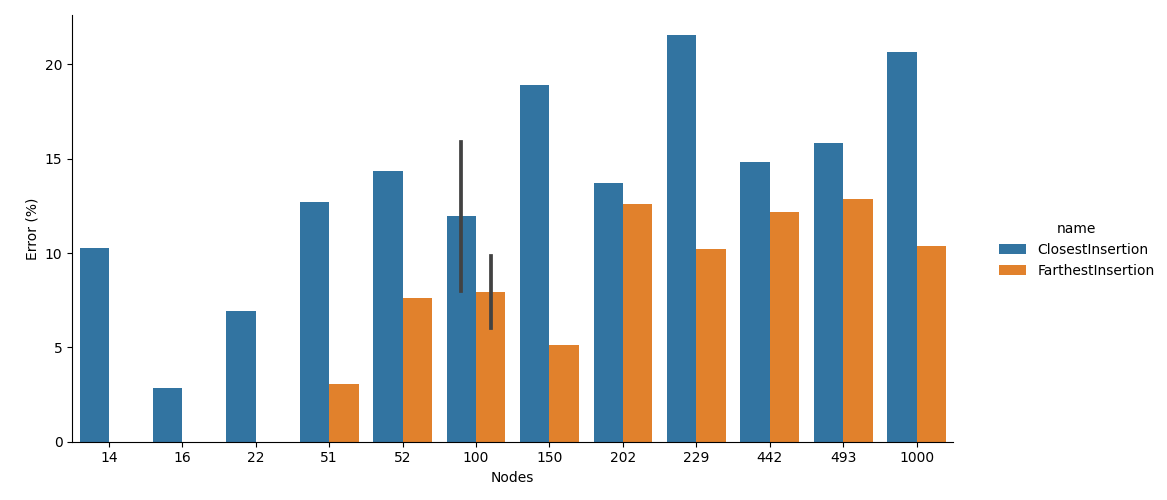
\includegraphics[width=0.9\textwidth]{./images/ClosestInsertion_vs_FarthestInsertion__approximation_error_.png}

    \caption{ClosestInsertion vs FarthestInsertion accuracy error scaling by nodes}
    \label{fig:closest-farthest-insertion-accuracy-error}
\end{figure}
